\documentclass[conference,a4paper]{IEEEtran}
\usepackage[T5]{fontenc}
\usepackage[utf8]{inputenc}
\usepackage[vietnamese]{babel}
\usepackage{amsmath,amssymb}
\usepackage{graphicx}
\usepackage{booktabs}
\usepackage{algorithm,algpseudocode}
\floatname{algorithm}{Thuật toán}
\usepackage{url}
\usepackage[hidelinks]{hyperref}

% Compile with pdfLaTeX + BibTeX. IEEEtran and Vietnamese fonts (vntex) required.
% Chapters 1–2 implemented by A; Chapter 3 remains B's pending work.
\newcommand{\todo}[1]{\textbf{[TODO: #1]}}

\title{Khai thác tập phổ biến bằng Eclat:\\Cài đặt Julia, đánh giá và ứng dụng Groceries -- Splice DNA}
\author{\IEEEauthorblockN{Nguyễn Đức Hưng \qquad Trần Thiên Phúc}
\IEEEauthorblockA{Môn Khai phá dữ liệu và ứng dụng\\
Khoa Công nghệ Thông tin, Trường Đại học Khoa học Tự nhiên, ĐHQG-HCM\\
Bản review phần A; Chương 3 chưa hoàn tất}}

\begin{document}
\maketitle

\begin{abstract}
Báo cáo trình bày ECLAT bằng Julia với hai biểu diễn tidsets: sorted lists và
BitVector. Cả hai dùng cùng DFS prefix extension và trả mọi frequent itemset cùng
support tuyệt đối. Phần cài đặt phân biệt rõ lịch DFS của nhóm với bottom-up trong
paper Zaki (2000), đồng thời cung cấp parser/writer SPMF và threshold chính xác.
Kiểm chứng kết hợp oracle vét cạn độc lập, dữ liệu ngẫu nhiên và output thực của
SPMF. Thực nghiệm trên Chess, Mushroom, Retail và T10I4D100K dùng sáu ngưỡng mỗi
CSDL, năm repetitions; so sánh end-to-end riêng với read+mine trong Julia đã warm.
Peak RSS được đo bằng hệ điều hành, cùng thí nghiệm Retail nested subsets và
synthetic transaction widths. Các bảng và hình sinh từ CSV/logs thực, không giới
hạn output để giảm thời gian. Phân tích tập trung vào mật độ tidsets, chi phí
intersection, allocation và ảnh hưởng runtime nền; không giả định BitVector luôn
có lợi trên dữ liệu thưa. Đây là bản review Chương 1--2 của thành viên A; Chương 3
về Groceries và Splice DNA thuộc thành viên B còn ở trạng thái template, nên PDF
chưa phải báo cáo nghiệm thu cuối của nhóm.
\end{abstract}

\begin{IEEEkeywords}
frequent itemset mining, Eclat, Julia, BitVector, association rules, splice DNA
\end{IEEEkeywords}

% Three main chapters as IEEE sections; do not use book/report \chapter commands.
\section{Chương 1: Cài đặt thuật toán ECLAT}
\label{sec:implementation}

\subsection{Bài toán và phạm vi cài đặt}
Khai thác tập phổ biến (frequent itemset mining, FIM) tìm các tổ hợp item xuất hiện
trong đủ số quan sát. Kết quả là đầu vào của bài toán luật kết hợp: cùng một tập
phổ biến có thể sinh nhiều luật có confidence và lift khác nhau~\cite{agrawal1994}.
Trong đồ án, thuật toán được viết bằng Julia, không gọi thư viện FIM để thực hiện
mining. SPMF chỉ đóng vai trò tham chiếu độc lập và đối tượng so sánh thời gian.
Hai backend của nhóm cùng trả mọi tập phổ biến và support tuyệt đối, gồm cả các
tập không đóng và không tối đại. Việc giữ đầy đủ kết quả cần thiết để tra support
của các tập con khi sinh luật, nhưng cũng làm chi phí bộ nhớ phụ thuộc output.

Gọi $D=(t_1,\ldots,t_n)$ là dãy $n$ giao dịch; $I$ là tập $m$ item phân biệt;
$t_i\subseteq I$ và $X\subseteq I$, $X\ne\emptyset$. Dùng dãy thay vì loại trùng
các giao dịch: hai giỏ hàng giống nội dung vẫn là hai quan sát độc lập. Tidset và
support count của $X$ được định nghĩa bởi
\begin{equation}
 T(X)=\{i\in\{1,\ldots,n\}:X\subseteq t_i\},\quad
 \sigma(X)=|T(X)|.
 \label{eq:support}
\end{equation}
Khi $n>0$, relative support là $s(X)=\sigma(X)/n$. Với minsup tương đối
$\theta\in(0,1]$, cài đặt dùng
\begin{equation}
 \tau=\max\{1,\lceil\theta n\rceil\},\qquad
 F=\{X\subseteq I:X\ne\emptyset,\ \sigma(X)\ge\tau\}.
 \label{eq:threshold}
\end{equation}
Dấu bằng được giữ: support đúng ngưỡng vẫn frequent. CSDL rỗng hoặc $\tau>n$
trả vector rỗng; không định nghĩa relative support bằng phép chia cho không.
API trong RAM chấp nhận giao dịch rỗng, vẫn tính nó trong $n$, còn blank line
trong file được xem là khoảng trắng và không tạo giao dịch. Chính sách khác nhau
này là tường minh, tránh thay đổi denominator khi đọc dữ liệu ứng dụng.

Ví dụ $\theta=0.07,n=100$ phải cho $\tau=7$. CLI phân tích chuỗi thập phân
thành \texttt{Rational\{BigInt\}}, rồi tính ceiling chính xác; không đi qua
Float64. Dạng \texttt{40\%} và \texttt{0.4} cùng biểu diễn $2/5$.
Không nhận scientific notation hay giá trị ngoài $(0,1]$ qua CLI. API mining nhận
absolute count nguyên dương, tách biệt quyết định ngưỡng khỏi thuật toán.

\subsection{Biểu diễn vertical và phân hoạch prefix}
Trong horizontal layout, mỗi hàng chứa các item của một transaction. Vertical
layout lưu danh sách TID cho từng item; TID là chỉ số 1-based sau bước chuẩn bị.
Công thức then chốt là
\begin{equation}
 T(X\cup Y)=T(X)\cap T(Y).
 \label{eq:intersection}
\end{equation}
Một TID nằm ở vế trái khi transaction chứa cả $X$ lẫn $Y$, đúng với điều kiện
nằm trong cả hai tập ở vế phải. Bởi vậy không cần quét toàn bộ horizontal database
để đếm từng candidate. Nếu $X\subseteq Y$ thì $T(Y)\subseteq T(X)$, suy ra
$\sigma(Y)\le\sigma(X)$. Đây là tính anti-monotone dùng để prune: candidate có
support nhỏ hơn $\tau$ không có frequent descendant.

Cố định item order theo ID tăng dần. Với prefix tăng $P$, các atom trong một lớp
có dạng $P\mathbin{\|}x$, trong đó $\|$ là phép nối tuple. Mỗi atom lưu key đầy
đủ và tidset chính xác của key; extension $x$ tăng theo thứ tự của lớp. Chỉ ghép
atom hiện tại với sibling đứng sau. Lớp con cho $P\mathbin{\|}x$ chứa các
$P\mathbin{\|}x\mathbin{\|}y$ đạt ngưỡng với $y>x$. Phân hoạch này vừa cung cấp
đường đi canonical vừa giới hạn số lớp trung gian phải xử lý đồng thời.

\subsection{Liên hệ với Zaki (2000) và lựa chọn adaptation}
Nguồn thuật toán chính là Zaki~\cite{zaki2000}: mục 4.1 trình bày support counting
qua tid-lists; mục 4.2 phân rã lattice theo prefix; mục 5.4 mô tả Eclat bằng
prefix equivalence và bottom-up search. Fig.~12 dựng các lớp con trước khi gọi
đệ quy. Nhóm giữ nguyên cơ sở giao tidsets và phân hoạch, đồng thời chọn duyệt
theo chiều sâu (depth-first search, DFS): xử lý hết một lớp con trước sibling.
Thuật toán~\ref{alg:dfs} phản ánh mã nhóm và không phải bản chép nguyên Fig.~12.
Tài liệu SPMF cũng mô tả một phiên bản Eclat theo DFS~\cite{spmf}.

Một lựa chọn khác liên quan $F_2$. Trong mã nhóm, các cặp singleton frequent được
giao trực tiếp trong RAM. Nhóm không triển khai bước vertical-to-horizontal
recovery và bộ đếm cặp tam giác của mục 5.1. Vì vậy kết quả giữ cùng ngữ nghĩa
FIM nhưng không được xem là tái tạo toàn bộ các tối ưu và kiến trúc lưu trữ của
paper. Không dùng diffsets, maximal-clique partitioning hay chỉ xuất maximal sets.
Ghi chú chi tiết và ánh xạ từng mục paper nằm trong \path{docs/paper-notes.md}.

\begin{algorithm}[tb]
\caption{DFS prefix extension chung cho hai backend}
\label{alg:dfs}
\begin{algorithmic}[1]
\Require Các atom $S$ có cùng prefix, tăng theo extension; ngưỡng $\tau$
\Function{DFS}{$S,\tau,F$}
\For{$i=1,\ldots,|S|$}
  \State $a\gets S_i$
  \State thêm $(a.key,\operatorname{support}(a.tids))$ vào $F$
  \State $C\gets[\ ]$
  \For{$j=i+1,\ldots,|S|$}
    \State $b\gets S_j$
    \State $U\gets\operatorname{intersect}(a.tids,b.tids)$
    \If{$\operatorname{support}(U)\ge\tau$}
      \State $K\gets a.key\mathbin{\|}\operatorname{last}(b.key)$
      \State thêm atom $(K,U)$ vào $C$
    \EndIf
  \EndFor
  \If{$C$ khác rỗng}
    \State \Call{DFS}{$C,\tau,F$}
  \EndIf
\EndFor
\EndFunction
\end{algorithmic}
\end{algorithm}

\subsection{ECLAT Basic: verticalization và phép giao}
Backend Basic ở \path{src/algorithm/baseline.jl}. Duyệt từng transaction theo
\texttt{enumerate}, thêm TID vào dictionary từ item đến \texttt{Vector\{Int\}}.
Validation đã bảo đảm mỗi item có tối đa một lần trong một transaction; TID được
thêm tăng dần nên lists tự sorted, không phải sort lại. Các singleton dưới
$\tau$ bị loại khỏi danh sách atom; các key còn lại được sort tăng ID. Một transaction
lặp nội dung vẫn được thêm với TID mới, đúng định nghĩa tại (\ref{eq:support}).

Phép \texttt{intersect\_tids} dùng hai con trỏ $i,j$, bắt đầu tại vị trí đầu của
hai lists $A,B$. Nếu $A_i=B_j$, ghi TID và tăng cả hai; nếu nhỏ hơn, chỉ tăng con
trỏ của giá trị nhỏ hơn. Dừng khi một list hết. Các phần tử đã đi qua không còn
khả năng khớp với phần suffix của list kia, nên quy tắc không bỏ sót giao. Mỗi
con trỏ tăng tối đa độ dài list; không dùng vòng lặp membership tuyến tính lồng
nhau. Hai input chỉ đọc; kết quả cấp phát mới, có size hint bằng độ dài list ngắn.
Cách này xử lý đúng cả giao rỗng lẫn một trong hai lists rỗng.

\begin{table}[tb]
\centering
\caption{Ví dụ tự xây dựng: horizontal và vertical layout, $n=4,\tau=2$.}
\label{tab:trace}
\begin{tabular}{clcl}
\toprule
TID & Transaction & Item & TID-list \\
\midrule
1 & $\{1,2,3\}$ & 1 & $[1,2,4]$ \\
2 & $\{1,3\}$ & 2 & $[1,3,4]$ \\
3 & $\{2,3\}$ & 3 & $[1,2,3]$ \\
4 & $\{1,2\}$ & & \\
\bottomrule
\end{tabular}
\end{table}

Theo Bảng~\ref{tab:trace}, ba singletons có support 3. Nhánh đầu emit $\{1\}$;
giao với item 2 cho $[1,4]$ và với item 3 cho $[1,2]$. Lớp prefix 1 gồm hai atom
frequent $\{1,2\}$ và $\{1,3\}$. Sau khi emit $\{1,2\}:2$, phép giao hai atom
con chỉ cho $[1]$: candidate $\{1,2,3\}$ có support 1 và bị prune. Quay lui,
emit $\{1,3\}:2$. Nhánh item 2 còn sinh $\{2,3\}:[1,3]$, cuối cùng emit item 3.
Kết quả có 6 itemsets. Ví dụ minh họa này khác fixture \texttt{basic.txt} thực tế,
có 5 transactions và 7 patterns tại 40\%; tách biệt hai ví dụ tránh gán nhầm expected.

\subsection{Kiểu dữ liệu, API và xử lý vào/ra}
Bảng~\ref{tab:types} tóm tắt các kiểu của schema v1.0.0. Hai backends dispatch từ
\texttt{mine} sang representation cụ thể, nhưng gọi chung
\texttt{enumerate\_class!}. Vì vậy ordering, phát candidate và pruning không bị
thay đổi giữa hai phép đo. Các vector atom và tidset trong hot loop có kiểu cụ thể;
key có độ dài thay đổi theo itemset theo hợp đồng dùng chung.

\begin{table}[tb]
\centering
\caption{Các kiểu dữ liệu thực tế trong implementation.}
\label{tab:types}
\begin{tabular}{ll}
\toprule
Kiểu & Nội dung chính \\
\midrule
\texttt{Itemset} & Tuple ID dương tăng, không trùng \\
\texttt{Pattern} & Canonical key và support tuyệt đối \\
\texttt{ListAtom} & Full key và sorted \texttt{Vector\{Int\}} \\
\texttt{BitsetAtom} & Full key và \texttt{BitVector} \\
\texttt{PreparedDataset} & Transactions, mapping và metadata \\
\bottomrule
\end{tabular}
\end{table}

API gọi \texttt{mine(transactions,min\_count)} với keyword
\texttt{backend=:list}; backend còn lại là
\texttt{:bitset}; trả \texttt{Vector\{Pattern\}}. Parser đọc numeric SPMF TXT,
bỏ blank và các dòng bắt đầu bằng \texttt{\#}, \texttt{\%}, \texttt{@}. Item không
dương, item lặp hoặc dòng không tăng bị reject; parser không âm thầm chuẩn hóa
lỗi. Input caller không bị thay đổi. Các bước chuẩn bị benchmark chuyển ID 0 về
ID dương được ghi nhận riêng ở Chương~\ref{sec:evaluation}.

Writer sắp theo độ dài, sau đó tuple items rồi ghi
\texttt{1 2 \#SUP: 3}. Output ổn định độc lập thứ tự DFS và bị từ chối nếu có key
lặp. Comparator đọc về dictionary key canonical và support nguyên; reject duplicate
output kể cả khi dòng có cùng support. Với fixture \texttt{basic.txt}, hai lựa chọn
CLI \texttt{--minsup 0.4} và \texttt{--min-count 2} cho cùng byte output. Các lệnh
chạy trong \path{scripts/mine.jl}; CLI bắt lỗi option trùng, thiếu tham số, hai dạng
support cùng lúc và output trùng input. Test round trip chạy cả hai backend.

\subsection{Tính đúng đắn và quản lý bộ nhớ}
\textit{Invariant về support.} Singleton tidsets đúng theo cách dựng từ từng TID.
Giả sử các atom ở một lớp chứa tidset đúng. Khi ghép hai atom cùng prefix,
(\ref{eq:intersection}) cho tidset chính xác của key union. Chỉ candidate đạt
$\tau$ được đưa vào lớp con, nên mọi Pattern được emit có support đúng và frequent.

\textit{Không trùng.} Một key canonical $x_1<\cdots<x_k$ chỉ có một chuỗi prefix
$x_1,x_1x_2,\ldots,x_1\cdots x_k$. Quy tắc chỉ ghép later siblings không cho đường
hoán vị hoặc sibling khác tạo lại cùng key. Không emit empty prefix.

\textit{Đầy đủ.} Nếu $X$ frequent thì mọi tập con cần cho các bước giao tạo prefix
của $X$ đều frequent. Chúng không thể bị prune. Theo quy nạp trên độ dài prefix,
DFS sẽ xét đúng extension tiếp theo và cuối cùng emit $X$. Như vậy thuật toán
xuất mọi frequent itemset, không chỉ các phần tử cực đại của lattice.

Mỗi candidate có tidset mới; không chia sẻ buffer mutable với parent. Khi đệ quy
trở về, lớp con hết được sử dụng có thể được garbage collector thu hồi. Tuy nhiên
các ancestor classes vẫn đang hoạt động; không áp dụng bound ``chỉ hai mức'' của
một lịch duyệt khác. Output vector giữ toàn bộ Patterns đến khi mining kết thúc;
writer cũng tạo vector được sắp thứ tự. Các phần này cùng tham gia peak RAM.

\subsection{Tối ưu BitVector}
Backend ở \path{src/algorithm/bitset.jl} đếm singletons trước, chỉ cấp bitmap cho
items đạt $\tau$, sau đó duyệt transactions lần nữa để đặt bit. Với $n$ giao dịch,
bit thứ $i$ bằng 1 khi item xuất hiện ở TID $i$. BitVector là mảng bit đóng gói
của Julia~\cite{juliaarrays}; phép \texttt{a .\& b} tạo giao mới và \texttt{count}
đếm bit được đặt. Cài đặt sử dụng API công khai, không thao tác trực tiếp internal
chunks. Các độ dài không chia hết cho word size được kiểm tra riêng.

Ở bước đệ quy, chỉ phép giao và hàm support khác Basic. Không dùng in-place AND
vào mask cha, không giới hạn độ dài pattern và không thay đổi item ordering để tạo
lợi thế benchmark. AND rồi count hiện là hai thao tác; chưa fuse chúng hay reuse
candidate buffers. Hai cách biểu diễn do đó có cùng cây liệt kê và cùng kết quả,
nhưng chi phí xử lý tidsets khác nhau. Correctness về ownership được kiểm bằng
repeated calls, invariance khi đảo transactions và oracle trên dữ liệu ngẫu nhiên.

\subsection{Phân tích thời gian và bộ nhớ}
Gọi $L=\sum_{i=1}^n|t_i|$, $m_1=|F_1|$, $C$ là tập candidate intersections thực
sự được thực hiện, và $w$ là số bit/word. Với $c\in C$, hai tidsets đầu vào là
$T_{c,a},T_{c,b}$. Basic có chi phí giao
\begin{equation}
 T_{\mathrm{join,list}}=O\!\left(\sum_{c\in C}
 (|T_{c,a}|+|T_{c,b}|)\right).
 \label{eq:list-cost}
\end{equation}
Verticalization cần $O(L)$ và sort IDs cần $O(m\log m)$. BitVector dựng masks với
chi phí $O(L+m_1\lceil n/w\rceil)$ ngoài sorting, còn tổng giao/count là
\begin{equation}
 T_{\mathrm{join,bit}}=O\!\left(|C|\lceil n/w\rceil\right).
 \label{eq:bit-cost}
\end{equation}
Hai công thức không bao gồm tất cả chi phí: validation và hashing input; tạo key;
constructor Pattern sort/validate key; GC; writer sort và serialization. Riêng
normalization các key có tổng bound $O(\sum_{X\in F}|X|\log|X|)$ và ghi output cần
ít nhất số item IDs $\sum_{X\in F}|X|$. Trường hợp mọi tập con frequent có
$|F|=2^m-1$; không có bound tuyến tính vô điều kiện. Các kết quả graph-theoretic
với giả thiết sparsity ở Appendix A của paper không thay thế phân tích cài đặt này.

Bộ nhớ gồm horizontal input $O(L)$, vertical data, active classes, một giao tạm và
output. Một list dùng khoảng $8|T|$ byte payload trên máy 64-bit, còn một bitmap
cần $8\lceil n/64\rceil$ byte cộng overhead object/array. So payload, điểm cân bằng
xấp xỉ $|T|/n=1/64$; đây chỉ là heuristic vì dictionary, allocation và cache còn
ảnh hưởng. Lists co ngắn khi đi sâu vào sparse intersections, bitmap vẫn dài $n$.
BitVector có thể giảm chi phí trên dense cases nhưng không được giả định luôn
nhanh hơn hoặc luôn giảm resident set size (RSS). Peak process RSS còn gồm runtime
và biên dịch just-in-time (JIT); dữ liệu
cấp phát tích lũy từ \texttt{@timed} là metric khác.

\subsection{Kiểm thử, association rules và tái lập}
Bộ kiểm thử mặc định bật cả hai backend và SPMF references. Oracle độc lập liệt
kê mọi subset của tối đa 12 items rồi đếm trực tiếp trên horizontal transactions;
không dùng phép giao của miner. Năm fixtures basic/dense/sparse/duplicates/boundary
được kiểm ở count 1, count 2, $n$ và $n+1$. Thêm 20 DB ngẫu nhiên seed 42,
CSDL/transaction rỗng, một item, ID không liên tiếp, database dày, input invalid,
caller ownership và các kích thước 63/64/65/127/128/129 giao dịch. Các test cuối
cho cả phần mining, schema, rules và CLI được lưu nguyên stdout.

Reference tại 40\% được tạo thực sự bằng SPMF 2.64b, pin JAR SHA-256, input hash,
output hash và lệnh trong manifest. Comparator xác minh toàn bộ key/support,
đếm missing, extra, wrong support; hai output rỗng vẫn là một trường hợp hợp lệ,
không tự suy correctness của các trường hợp có output từ ví dụ rỗng. Trên benchmark,
runner còn đối chiếu từng cấu hình trước khi đo và kiểm output của từng repetition.

Helper \texttt{association\_rules} dùng support dictionary đầy đủ, xét mọi phân
hoạch $X=A\cup B$ với hai phía khác rỗng, rời nhau. Confidence được lọc bằng tỉ số
counts chính xác trước khi xuất Float64; subset support thiếu là lỗi. Duyệt tập con
đệ quy không phụ thuộc bitmask có số bit cố định. Luật được sort theo lift,
confidence, support giảm dần, rồi length và keys tăng dần theo schema. Test dùng
PreparedDataset để gọi mine và kiểm cả consequent nhiều item. Hai preprocessing
pipelines Groceries/DNA thuộc Chương 3 vẫn cần thành viên B hoàn thiện; việc helper
chạy đúng không được dùng để tuyên bố ứng dụng trên dữ liệu thực đã hoàn thành.

\section{Chương 2: Thực nghiệm và đánh giá}
\label{sec:evaluation}

\subsection{Câu hỏi thực nghiệm và thiết lập}
\todo{A nêu câu hỏi: correctness, ảnh hưởng minsup, dense/sparse, BitVector,
scalability và transaction length. B review tính công bằng.}
\todo{Điền CPU, RAM, OS, Julia/Java/SPMF, thread count, seed, warm-up, số lần lặp,
median/spread, timeout và phạm vi timer. Phân biệt internal read+mine với
end-to-end wall-clock; không so hai phạm vi khác nhau như một metric.}

\subsection{Dữ liệu benchmark}
\begin{table}[htbp]
\centering
\caption{Thống kê trên đúng file benchmark dùng trong thí nghiệm; các ô chờ đo.}
\label{tab:datasets}
\begin{tabular}{lrrr}
\toprule
CSDL & $n$ & $m$ & Width TB \\
\midrule
Chess & -- & -- & -- \\
Mushroom & -- & -- & -- \\
Retail & -- & -- & -- \\
T10I4D100K & -- & -- & -- \\
\bottomrule
\end{tabular}
\end{table}
Trong Bảng~\ref{tab:datasets}, $n$ là số giao dịch, $m$ là số item phân biệt và width
là số item/giao dịch. \todo{Bổ sung nguồn snapshot HF/Kaggle, version/hash, license,
preprocessing và đặc điểm dense/sparse; tính số từ file thật.}

\subsection{Đối chiếu correctness với SPMF}
\todo{B so đầy đủ itemset/support cho từng CSDL/minsup; bảng n_patterns,
missing, extra, wrong support và exact match rate. Nêu denominator, trường hợp
output rỗng và phân tích mọi sai khác. Không chỉ so tổng số pattern.}

\subsection{Runtime và output size theo minsup}
\todo{A chèn bốn đồ thị runtime (basic, BitVector, SPMF), 5--7 ngưỡng giảm dần/tập;
median + spread, đơn vị, legend, caption và tham chiếu từng hình trong lời văn.
Chèn output-size curves, giải thích bằng intersection và candidate/output growth.}

% Example only: replace path after a real run; do not insert fabricated figures.
% \begin{figure}[htbp]
% \centering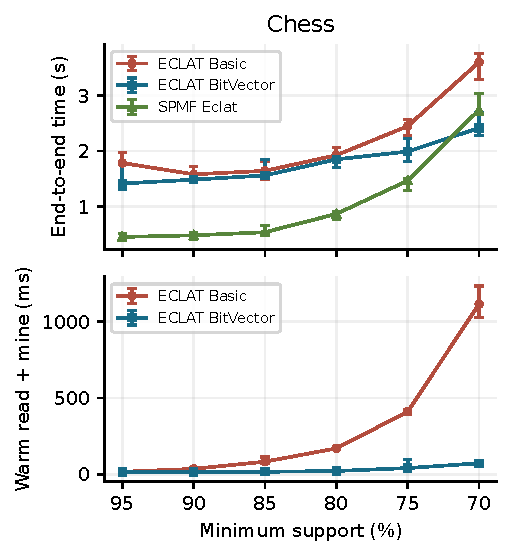
\includegraphics[width=\columnwidth]{figures/runtime-chess.pdf}
% \caption{Runtime trên Chess theo minsup, cùng phạm vi đo; TODO số lần lặp.}
% \label{fig:runtime-chess}
% \end{figure}

\subsection{Peak RAM và hiệu quả tối ưu}
\todo{A đo peak RSS basic/BitVector tại minsup trung bình của từng dataset.
Nêu công cụ OS và vòng đời process; không coi allocations là peak memory hoặc
so RSS với heap log. Bổ sung speedup và memory reduction từ số đo thật.}

\subsection{Scalability và độ dài giao dịch}
\todo{Retail: nested subsets 10/25/50/75/100\%, relative minsup cố định, tính
absolute count theo n thực. Vẽ runtime theo n, kèm output size và giới hạn sampling.}
\todo{Synthetic: n, m, seed, minsup cố định; transaction widths tăng dần; trình bày
runtime/output, mô tả generator mẫu và khác biệt với generator trong paper.}

\subsection{Thảo luận, hạn chế và tối ưu tiếp theo}
\todo{Giải thích xu hướng bằng mô tả thuật toán và complexity; nêu trường hợp
BitVector có lợi/bất lợi, JIT/JVM, I/O, warm-up, timeout/OOM và giới hạn phần cứng.}
\todo{Đề xuất ít nhất 2 hướng tối ưu cụ thể có cơ sở: ví dụ adaptive list/bitset,
buffer reuse, ordering/early-stop. Phân biệt điều đã đo với giả thuyết tương lai.}

\ifdefined\MemberAOnly
% Explicit A-only review; the team's complete three-chapter source stays intact.
\else
\section{Chương 3: Ứng dụng thực tế}
\label{sec:applications}

\subsection{Groceries: chuyển đổi giao dịch và khai thác}
\todo{B mô tả nguồn Groceries, snapshot/license, schema raw, thống kê trước/sau;
giải thích một basket là một transaction, item mapping, duplicate policy.}
\todo{Nêu minsup/minconf sau pilot và lý do; chạy basic/BitVector của nhóm,
không dùng output thư viện FIM cho kết quả ứng dụng.}

Với $A,B$ là hai itemset khác rỗng, rời nhau, xét luật $A\Rightarrow B$:
\begin{align}
\operatorname{supp}(A\Rightarrow B)&=\sigma(A\cup B)/n,\\
\operatorname{conf}(A\Rightarrow B)&=\sigma(A\cup B)/\sigma(A),\\
\operatorname{lift}(A\Rightarrow B)&=\operatorname{conf}(A\Rightarrow B)/(\sigma(B)/n).
\end{align}
$n$ là số basket; $\sigma$ được định nghĩa tại Eq.~\ref{eq:support}.
\todo{A/B giải thích lọc minsup/minconf, sinh luật, tie-break và chọn top-10 theo lift.}

\subsection{Groceries: kết quả và ý nghĩa kinh doanh}
\todo{B điền bảng top-10, decoded product names, support, confidence, lift và counts.
Giải thích ít nhất 3 luật với gợi ý thực tế; phân tích support thấp và tránh suy
nhân quả từ co-occurrence. Gắn artifact CSV và lệnh tái lập.}

\subsection{Splice DNA: dữ liệu và mã hóa 12 vị trí}
Dữ liệu UCI Splice~\cite{splice} có sequence DNA và ba nhãn EI, IE, N.
\todo{B trình bày provenance và counts theo lớp từ file thực; giải thích EI/IE/N.}
Theo kế hoạch, mỗi sequence được chuyển thành transaction từ 12 vị trí.
\todo{Xác nhận cửa sổ đề xuất $-6,\ldots,-1,+1,\ldots,+6$, chỉ số Julia 25:36;
item là cặp (vị trí, base), mapping ổn định, nhãn lớp giữ riêng.}
\todo{Giải thích ambiguity D/N/S/R, chính sách xử lý, số sample bị loại theo lớp;
phân biệt nhãn N với base N. Không coi tập base không vị trí là cùng representation.}

\subsection{Splice DNA: pattern 2--4 item và so sánh EI/IE/N}
\todo{Chạy cài đặt nhóm theo lớp; minsup relative dùng denominator của lớp.
Mine đầy đủ, sau đó lọc độ dài 2--4 để trình bày; thống nhất candidate across classes.}
\todo{B điền bảng decoded patterns, count và relative support từng lớp,
chênh lệch support, criterion chọn. Đếm trực tiếp candidate nếu không có trong
frequent output lớp khác; không tự gán support 0.}
\todo{Diễn giải co-occurrence quanh splice, imbalance, window/threshold selection
và ambiguity; không kết luận cơ chế sinh học hoặc accuracy classifier chưa đo.}

\subsection{Khả năng tái lập, hạn chế và kết luận}
\todo{B mô tả cold-run Colab: raw data, code chuẩn bị, mapping/config, miner, bảng,
figures. A/B tổng hợp kết quả thật hai ứng dụng, giới hạn và bước tiếp theo.
Kết luận ngắn bao quát cả ba chương, không thay kết luận bằng checklist công việc.}

\fi

\bibliographystyle{IEEEtran}
\bibliography{references}

% Optional appendix: raw configs, extra plots, test logs and reproducibility.
% References and appendices do not count toward the required 10–15 body pages.
\end{document}
